\section{Accountancy}
\label{sec:accountancy}

The accountancy package contains functionality supporting book keeping.
\code{AccountancyEntry} is a representation of an accounting entry.
\code{Accountancy} aggregates \code{AccountancyEntry}s.
Every \code{AccountancyEntry} is uniquely identified by an \code{AccountancyEntryIdentifier}.
\\

\code{PersistentAccountancyEntry} implements \code{AccountancyEntry} and serves as persistence entity, while \code{PersistentAccountancy} implements \code{Accountancy} and provides transparent access to the JPA layer.
\code{AccountancyEntryIdentifier} is used as primary key attribute, when entities are stored in the database.
\\

By implementing and sub-classing the \code{AccountancyEntry} interface, the notion of different accounts, as known from double-entry bookkepping, can be realised.
As can be seen in Figure~\ref{accountancy_overview}, \code{PersistentAccountancyEntry} is sub-classed to create a second ``account'' used to store payment information, namely \code{ProductPaymentEntry}.
\begin{figure}
	\centering
  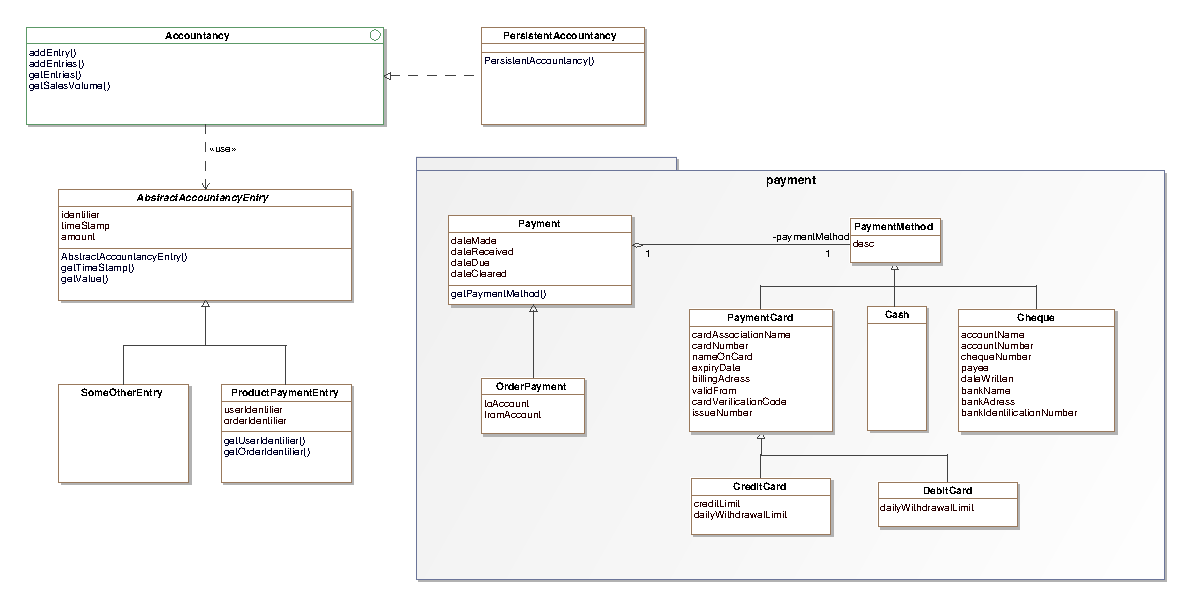
\includegraphics[width=1.0\textwidth]{images/Accountancy_Overview.eps}
	\label{accountancy_overview}
	\caption{Accountancy - Class Overview}
\end{figure}

Payment information also includes a user identifier referencing the buyer, an order identifier referring to the \code{Order} which was payed, and a \code{PaymentMethod} describing the money transfer.
The attributes are named \code{userIdentifier}, \code{orderIdentifier}, and \code{paymentMethod} respectively.
The inheritance hierarchy of \code{PaymentMethod} is depicted in Figure \ref{payment_overview}.

\begin{figure}
\centering
  \includegraphics[width=1.0\textwidth]{images/Payment_Overview.eps}
	\label{payment_overview}
	\caption{Payment - Class Overview}
\end{figure}

To create a new account, \code{AccountancyEntry} has to be sub-classed.
Every (persisted) object of such a class belongs to the same account.
Accessing per-account entries is facilitated by specifiying the desired class type when calling \code{get()} or \code{find()} methods of \code{Accountancy} as explained in Section \ref{jpa-types}.
